% reality/construction_and_realization-DE.tex
\chapter{Bau und physische Realisierung}
\label{chap:construction-and-realization}

Dieses Kapitel beantwortet, wie ein ingenieurtechnischer Zielzustand unter
Bau- und Instandhaltungsbedingungen zum physisch gebauten Eisenbahnzustand
wird. Es begründet die im Teil Realität verwendete Sicht des
Realisierungsoperators und klärt die Folgen für Laufzeitrekonstruktion und
realisierungsbewussten Entwurf.

Die Eingangsfrage ist deshalb vergleichend: Was ändert sich, wenn ein
analytischer Zielzustand in einen realisierten Zustand transformiert wird?

\begin{figure}[htbp]
\centering
% figures/reality/target_vs_realized_geometry-DE.tex
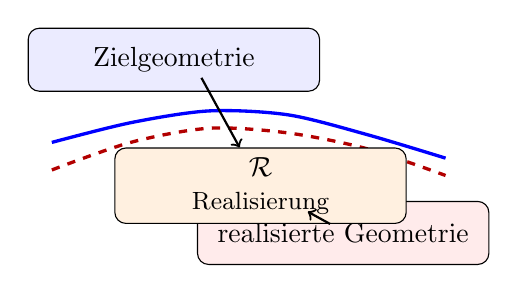
\begin{tikzpicture}[
  x=1cm,y=1cm,
  box/.style={draw, rounded corners, align=center, minimum width=3.7cm, minimum height=0.8cm},
  arrow/.style={->, thick}
]
\draw[very thick, blue] plot[smooth] coordinates {(0,0) (1,0.25) (2,0.4) (3,0.35) (4,0.1) (5,-0.2)};
\draw[very thick, red!70!black, dashed] plot[smooth] coordinates {(0,-0.35) (1,0.0) (2,0.18) (3,0.12) (4,-0.08) (5,-0.42)};
\node[box, fill=blue!8] at (1.55,1.05) {Zielgeometrie};
\node[box, fill=red!8] at (3.7,-1.15) {realisierte Geometrie};
\node[box, fill=orange!12] (R) at (2.65,-0.55) {$\mathcal R$\\\small Realisierung};
\draw[arrow] (1.9,0.82) -- (R);
\draw[arrow] (R) -- (3.25,-0.88);
\end{tikzpicture}

\caption{Zielgeometrie und realisierte Geometrie, verbunden durch den Realisierungsoperator.}
\label{fig:target-vs-realized-geometry}
\end{figure}

Die Abbildung zeigt diesen Vergleich auf einen Blick und motiviert die in den
folgenden formalen Abschnitten verwendete Operatorformulierung.

Dieses Kapitel ist der kanonische Ort der physischen Realisierung im Teil
Realität. Physische Realisierung transformiert den ingenieurtechnischen
Zielzustand unter Bau-, Instandhaltungs- und strukturellen Bedingungen in den
physisch gebauten Zustand.

\begin{principle}[Realisierungsprinzip]
\label{princ:realization-principle}
In AIM ist die physische Realisierung eine Operatorebene, die Zielzustände in
physisch realisierte Zustände transformiert.
\end{principle}

\section{Physische gegenüber metrischer Realisierung}

Metrische Realisierung (\cref{chap:metric-realization}) definiert messbaren
Einbettungskontext. Physische Realisierung beschreibt die Wirkungen von Bau
und Instandhaltung auf die gebaute Infrastruktur. Beide Ebenen sind gekoppelt,
aber verschieden.

\begin{definition}[Realisiertes Alignment]
\label{def:realized-alignment}
Das realisierte Alignment ist die physisch gebaute Eisenbahngeometrie,
bezeichnet durch
\[
\gamma_{\mathrm{real}}(s).
\]
\end{definition}

\begin{definition}[Realisierte Krümmung]
\label{def:realized-curvature}
Die realisierte Krümmung ist
\[
\kappa_{\mathrm{real}}(s)=\frac{\dd\theta_{\mathrm{real}}}{\dd s}.
\]
\end{definition}

\section{Sicht des Realisierungsoperators}

\[
x_{\mathrm{real}}=\mathcal R(x_{\mathrm{target}}),
\]
wobei \(\mathcal R\) der kanonische Realisierungsoperator ist
(\cref{def:realization-operator}).

Realisierungsfehler können in zustandsabhängigen Räumen bewertet werden. Ein
krümmungsbasiertes Maß lautet
\[
E_{\kappa}
=
\int_0^L\left(\kappa_{\mathrm{real}}-\kappa_{\mathrm{target}}\right)^2\,\dd s.
\]

\section{Bau- und Anpassungsprozess}

Bau und Instandhaltung sind iterative lokale Prozesse.

Die folgenden Definitionen und Propositionen formalisieren diesen praktischen
Ablauf als iterativen Realisierungsprozess, dessen Fixpunktsicht die
Ingenieurpraxis mit der Operatorsemantik verbindet.

\begin{definition}[Anpassungsoperator]
\label{def:adjustment-operator}
Der Anpassungsoperator \(\mathcal A\) bezeichnet eine lokale Bau- oder
Instandhaltungsaktualisierung, die auf einen bestehenden Alignment-Zustand
angewandt wird.
\end{definition}

\begin{definition}[Iterative Realisierung]
\label{def:iterative-construction-realization}
Ausgehend von \(\gamma_0\) kann ein iterativer Realisierungsprozess dargestellt
werden durch
\[
\gamma_{k+1}=\mathcal A_{\gamma_{\mathrm{target}}}(\gamma_k).
\]
\end{definition}

\begin{definition}[Realisiertes Alignment als Grenzwert]
\label{def:realized-alignment-limit}
Konvergiert dieser Prozess, gilt
\[
\gamma_{\mathrm{real}}=\lim_{k\to\infty}\gamma_k.
\]
\end{definition}

\begin{proposition}[Fixpunktinterpretation]
\label{prop:realization-fixed-point}
Konvergiert die iterative Realisierung gegen \(\gamma_{\mathrm{real}}\) und
ist \(\mathcal A_{\gamma_{\mathrm{target}}}\) in \(\gamma_{\mathrm{real}}\)
stetig, dann gilt
\[
\gamma_{\mathrm{real}}=
\mathcal A_{\gamma_{\mathrm{target}}}(\gamma_{\mathrm{real}}).
\]
\end{proposition}

\begin{proof}
Grenzübergang auf beiden Seiten von
\(\gamma_{k+1}=\mathcal A_{\gamma_{\mathrm{target}}}(\gamma_k)\) und
Stetigkeit im Grenzwert ergeben
\(\gamma_{\mathrm{real}}
=\lim_{k\to\infty}\mathcal A_{\gamma_{\mathrm{target}}}(\gamma_k)
=\mathcal A_{\gamma_{\mathrm{target}}}(\gamma_{\mathrm{real}})\).
\end{proof}

Auf die Stetigkeit kann nicht verzichtet werden. Auf \(\R\) erzeugt die
Abbildung mit \(\mathcal A(0)=1\) und \(\mathcal A(x)=x/2\) für \(x\neq0\)
Orbits, die gegen \(0\) konvergieren, obwohl \(0\) kein Fixpunkt ist.

\section{Abtastung, Lokalität und Filterung}

\begin{definition}[Kontrollpunkte]
\label{def:control-points}
Es seien
\[
0=s_0<s_1<\dots<s_N=L
\]
die Kontrollpunktstationen, die in Realisierungs- und
Instandhaltungsabläufen verwendet werden.
\end{definition}

\begin{proposition}[Prinzip adaptiver Abtastung]
\label{prop:adaptive-sampling-principle}
Die Abtastdichte soll in Bereichen starker Krümmungsänderung zunehmen.
\end{proposition}

\begin{definition}[Lokale Korrektur]
\label{def:local-correction}
Eine lokale Korrekturform ist
\[
\mathcal A_{\gamma_{\mathrm{target}}}(\gamma)
=
\gamma+\Delta(\gamma,\gamma_{\mathrm{target}}).
\]
\end{definition}

\begin{proposition}[Lokalität]
\label{prop:adjustment-locality}
Anpassung hängt vom lokalen Nachbarschaftskontext und nicht vom globalen
Alignment-Zustand ab.
\end{proposition}

\begin{definition}[Kernelbasierte Anpassung]
\label{def:kernel-based-adjustment}
Ein linearisiertes lokales Modell lautet
\[
(\mathcal A_{\gamma_{\mathrm{target}}}\gamma)(s)
=
\gamma(s)+
\int_I K(s,\sigma)
\bigl(\gamma_{\mathrm{target}}(\sigma)-\gamma(\sigma)\bigr)
\,\dd\sigma.
\]
\end{definition}

\begin{definition}[Diskretes Anpassungsmodell]
\label{def:discrete-adjustment-model}
Für Kontrollpunkte gilt
\[
\gamma_i^{(k+1)}
=
\gamma_i^{(k)}+
\sum_j K_{ij}\left(\gamma_j^{\mathrm{target}}-\gamma_j^{(k)}\right).
\]
\end{definition}

\begin{proposition}
\label{prop:realization-low-pass}
Physische Realisierung wirkt näherungsweise als Tiefpassfilter auf Krümmung
und verwandte hochfrequente Komponenten.
\end{proposition}

\begin{principle}[Prinzip des Realisierungsfilters]
\label{princ:realization-filter}
Bau und Instandhaltung transformieren den Zielzustand durch physische
Abtastung, Maschinenreaktion und strukturelle Filterung.
\end{principle}

\section{Folgen für Laufzeit und Optimierung}

Die Realisierungsebene ist mit dünn besetzter Modellierung und
Laufzeitbewertung vereinbar: Realisierte Geometrie kann als gemessene
Stichproben, rekonstruierter Laufzeitzustand oder mit dünn besetzten Modellen
kompatible Approximation interpretiert werden.

Dieser Abschnitt führt damit von der Baumechanik zur ingenieurtechnischen
Folge: Die Leistung des realisierten Zustands wird zum maßgeblichen
Entwurfskriterium für die nachgelagerte Optimierung.

\begin{principle}[Kompatibilität dünn besetzter Realisierung]
\label{princ:sparse-realization-compatibility}
Realisierungsbewusste Abläufe müssen mit dünn besetzten und
laufzeitbezogenen Zustandsarchitekturen kompatibel bleiben.
\end{principle}

\begin{definition}[Realisierungsbewusste Zielfunktion]
\label{def:realization-aware-objective}
Ein realisierungsbewusstes Entwurfsziel kann geschrieben werden als
\[
\min_{x_{\mathrm{target}}}J\bigl(\mathcal R(x_{\mathrm{target}})\bigr).
\]
\end{definition}

\begin{proposition}[Prinzip realisierungsbewussten Entwurfs]
\label{prop:realization-aware-design}
Das maßgebliche Entwurfskriterium ist die Leistung des realisierten Zustands,
nicht allein die analytische Glattheit des Zielzustands.
\end{proposition}

\begin{definition}[Physischer Entwurfsraum]
\label{prop:physical-design-space}
Der physische Entwurfsraum ist das Bild des Realisierungsoperators
\(\mathcal R\) über den zulässigen Zielzuständen.
\end{definition}

Ob \(\mathcal R\) einen Bauprozess angemessen modelliert, ist eine
getrennte empirische Frage; die Definition beantwortet sie nicht.

\section{Verbindung zu AIM}

\begin{summary}
Bau und physische Realisierung verbinden den ingenieurtechnischen Zielzustand
mit dem Zustand der gebauten Infrastruktur.

In AIM ist physische Realisierung eine ausdrückliche nachgelagerte Ebene, die
konstruktive Semantik und metrischen Realisierungskontext verwendet und
realisierten Zustand für Messung, Laufzeitrekonstruktion und
ingenieurtechnische Interpretation erzeugt.

Das folgende Realitätskapitel kann den Ziel--Realisiert-Vergleich daher als
evidenzbasierte Bewertungsebene behandeln, die auf diesem Fundament des
Realisierungsoperators aufbaut.
\end{summary}
